\subsection{Datasets}

There are multiple datasets available which facilitate the interaction with Wikipedia, and due to the massive amount of data, it is important to have an organized and manageable representation of this data in our own servers for processing. 

\begin{figure}[H]
  \centering 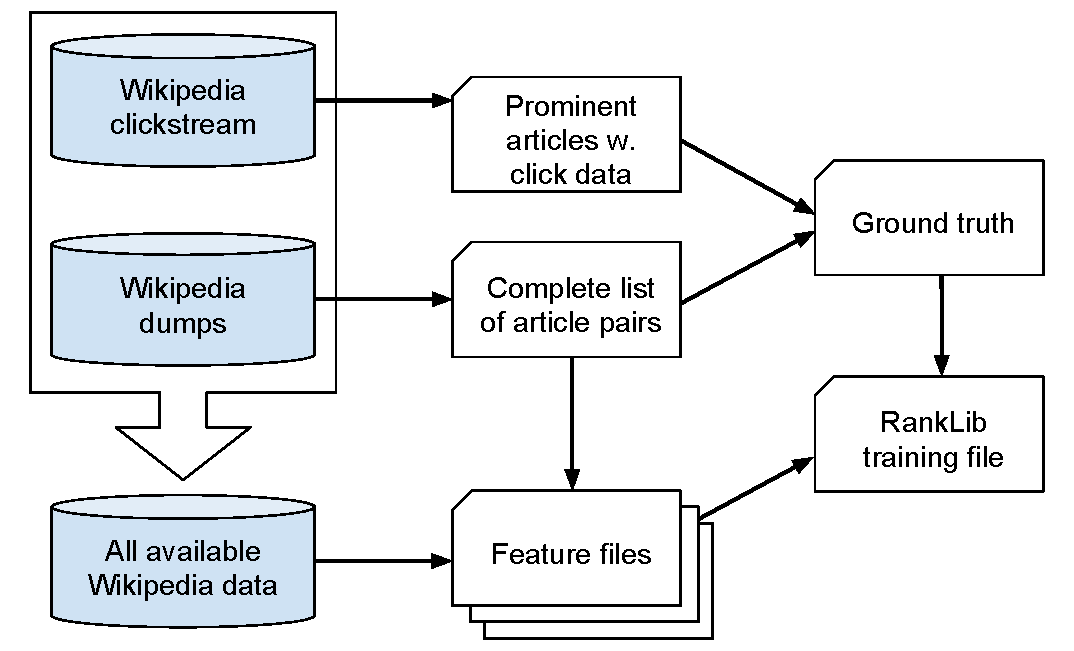
\includegraphics[width=0.49\textwidth]{images/process_small}
  \caption{Overall flow of data in the process of generating input for a supervised ranking model}
  \label{fig:process}
\end{figure}

Figure \ref{fig:process} illustrates the overall flow of data processing from the core datasets (sect. \ref{sec:wikidump} - \ref{sec:clickstream}) to the fully prepared RankLib file for use as an input to the algorithms described in sect. \ref{sec:ranklib}. We extract a subset of the articles and article pairs from the core datasets to create the ground truth (sect. \ref{sec:groundtruth}). By combining (merging tuples of) the ground truth and the features we describe in sect. \ref{sec:features}, we can construct the RankLib file, where we have tuples of feature values with associated rank.
% * <roelcastanomoreno@gmail.com> 2016-05-31T12:03:53.269Z:
%
% > By combining the ground truth with the features we describe in sect. \ref{sec:features}
%
% Its a bit confusing, what does combining mean?
%
% ^ <philip@thruesen.dk> 2016-06-01T16:51:14.075Z:
%
% added "(merging tuples of)". Perhaps it makes more sense then?
%
% ^ <jarekcechak@gmail.com> 2016-06-02T08:12:25.114Z.

\subsubsection{Wikipedia Dumps}
\label{sec:wikidump}
The most significant data source is the English Wikipedia database dump, which is released at least once a month, and contains a complete copy of the text and meta-data of current revisions of all articles in XML format. The English Wikipedia has more than 5 million articles, reaching a total of 50GB of text. Regarding links, even if only the top 1000 articles in Wikipedia are taken into account, there are a total of 250,000 outgoing links, which is the reason it was necessary to only focus on a subset of articles.

\subsubsection{Wikipedia Clickstream}
\label{sec:clickstream}
The Wikipedia Clickstream \cite{wulczyn} project contains datasets of $(referer, resource)$  pairs of articles describing user navigation and raw counts on the volume of traffic through the article pairs. This pairs are extracted from the request logs of Wikipedia, in which the referer is an HTTP header field that identifies the webpage from which the resource was requested. Requests for redirect articles are mapped to the articles they redirect to. Typical referral sites like Google or Facebook are also included and crawler-traffic has been filtered from the raw data. Any $(referer, resource)$   pair with less than 10 clicks has been removed from the dataset. In the March 2016 release, 6.8 billion requests were processed for a total of 25 million pairs.